% Generated from main.typ. Typst is authoritative; regeneration overwrites this file.
\documentclass{qlnotes-export}

\title{MATH 597: Measure Theory}
\subtitle{Typst-first course notes and worked homeworks}
\author{Qiulin Fan}
\date{Winter 2025}

\begin{document}
\mainmatter
\chapter{Homework 11: on regular Borel measure and functions of bounded variation (36/40)}\label{homework-11-on-regular-borel-measure-and-functions-of-bounded-variation-3640}

\section{Measurability of densities of measures}\label{measurability-of-densities-of-measures}

Suppose \(\mu\) is a regular (positive) Borel measure on \({\mathbb{R}}^{n}\).

\begin{itemize}
\item
  Prove that the functions \(\bar{f}:{\mathbb{R}}^{n}\rightarrow\lbrack 0, + \infty\rbrack\) and \(\underset{¯}{f}:{\mathbb{R}}^{n}\rightarrow\lbrack 0, + \infty\rbrack\) defined by

  \[\bar{f}(x) := \operatorname{lim\, sup}\limits_{r\rightarrow 0 +}\frac{\mu(B(x,r))}{m(B(x,r))},\quad\text{and}\quad\underset{¯}{f}(x) := \operatorname{lim\, inf}\limits_{r\rightarrow 0 +}\frac{\mu(B(x,r))}{m(B(x,r))}\]

  where \(m\) denotes Lebesgue measure, are Borel measurable.
\item
  Prove that the set

  \[A = \left\{ {x \in {\mathbb{R}}^{n} \mid \ \text{the limit}\lim\limits_{r\rightarrow 0 +}\frac{\mu(B(x,r))}{m(B(x,r))}\ \text{exists in}\lbrack 0, + \infty\rbrack\text{)}} \right\}\]

  is Borel measurable.
\item
  Give an example where \(A \neq {\mathbb{R}}^{n}\).
\end{itemize}

\emph{Hint}: we are taking the limsup over an uncountable set, so you probably need to use some properties of the functions \(r\mapsto\mu(B(x,r))\) and \(r\mapsto m(B(x,r))\), in addition to properties of \(x\mapsto\mu(B(x,r))\) and \(x\mapsto m(B(x,r))\).

\begin{proof}

\textbf{of (a):} We prove a lemma:

% qlnotes: kind=lemma; id=lem-hw11-on-regular-borel-measure-bv-lemma-001; concepts=lemma-001
\begin{lemma}\label{lem-hw11-on-regular-borel-measure-bv-lemma-001}

For regular positive Borel measure \(\mu\) on \({\mathbb{R}}^{n}\), fixing \(r > 0\), \(x\mapsto\mu(B(x,r))\) is Borel measurable.

\end{lemma}

\textbf{Proof of Lemma:} We recall

\[\mu(B(x,r)) = \int\chi_{B(x,r)}\, d\mu = \int\chi_{B(x,r)}(y)\, d\mu(y)\]

We define

\[f(x,y) = \chi_{B(x,r)}(y)\]

which is a function from \({\mathbb{R}}^{n} \times {\mathbb{R}}^{n}\rightarrow{\mathbb{R}}\), and takes value between \(0\) and \(1\).\\
Thus for \(a \geq 1\),

\[f^{- 1}((a,\infty)) = \varnothing \in \mathcal{B}({\mathbb{R}}^{n}) \otimes \mathcal{B}({\mathbb{R}}^{n})\]

for \(a < 0\),

\[f^{- 1}((a,\infty)) = f^{- 1}(\left\{ {0,1} \right\}) = {\mathbb{R}}^{n} \times {\mathbb{R}}^{n} \in \mathcal{B}({\mathbb{R}}^{n}) \otimes \mathcal{B}({\mathbb{R}}^{n})\]

For \(0 \leq a < 1\), \(f^{- 1}((a,\infty)) = f^{- 1}(\left\{ 1 \right\})\). Note this set is:

\[f^{- 1}((a,\infty)) = \left\{ {(x,y) \in {\mathbb{R}}^{n} \times {\mathbb{R}}^{n}:y \in B(x,r)} \right\} = \left\{ {(x,y) \in {\mathbb{R}}^{n} \times {\mathbb{R}}^{n}: \parallel x - y \parallel < r} \right\}\]

Since \(g:(x,y)\mapsto \parallel x - y\underset{2}{\parallel}\) is continuous function, and

\[f^{- 1}((a,\infty)) = \left\{ {(x,y) \in {\mathbb{R}}^{n} \times {\mathbb{R}}^{n}: \parallel x - y \parallel < r} \right\} = g^{- 1}(r)\]

is open, since it is preimage of an open set, under a continuous function.\\
Thus

\[f^{- 1}((a,\infty)) \in \mathcal{B}({\mathbb{R}}^{2n}) = \mathcal{B}({\mathbb{R}}^{n}) \otimes \mathcal{B}({\mathbb{R}}^{n})\]

Thus \(f\) is Borel measurable function, and since it is nonnegative, \(f \in L^{+}({\mathbb{R}}^{2n})\), thus by \textbf{Tonelli's Theorem},

\[x\mapsto\int f_{x}(y)\, d\mu(y) = \mu(B(x,r))\quad\text{is Borel measurable}\]

finishing the proof of Lemma.\\
Define for \(r > 0\)

\[f_{r}(x) := \frac{\mu(B\left( {x,r} \right))}{m(B\left( {x,r} \right))}\]

Notice that for each \(r\), \(m(B(x,r)) = c_{n}r^{n} > 0\) is constant regardless of \(x\), so \textbf{\(f_{k}\) is Borel measurable} as a product of a Boreal measurable function and a constant.\\
\strut ~So

\[\bar{f}(x) = \operatorname{lim\, sup}\limits_{r\rightarrow 0^{+}}f_{r}(x) = \lim\limits_{\epsilon > 0}\sup\limits_{0 < r < \epsilon}f_{r}(x)\]

For fixed \(\epsilon > 0\), we define \(h_{\epsilon}(x): = \sup_{0 < r < \epsilon}f_{r}(x)\), then for \(a \in {\mathbb{R}}\), we have

\[h_{\epsilon}((a,\infty)) = \bigcup\limits_{0 < r < \epsilon}f_{r}((a,\infty)) = \bigcup\limits_{0 < r < \epsilon,r \in {\mathbb{Q}}}f_{r}((a,\infty))\]

is Bore measurable, Thus \(h_{\epsilon}\) is a Borel measurable function, then

\[\bar{f} = \lim\limits_{\epsilon > 0}h_{\epsilon} = \lim\limits_{n\rightarrow\infty}h_{\frac{1}{n}}\]

is a Borel measurable function as limit of a seq of Borel measurable functions. 这里注意: Reducing limup (or liminf) over an uncountable sets to a countable one requires upper/lower semicontinuity. 因而我们需要说明一下 \(f_{r}\) 是 right ctn in r 的. Same trick is applied to \(\underset{¯}{f}\). We set \(g_{\epsilon}(x): = \inf_{0 < r < \epsilon}f_{r}(x)\) and have \(\underset{¯}{f}(x) = \lim_{n\rightarrow\infty}g_{\frac{1}{n}}\) is Borel measurable, finishing the proof.

\end{proof}

\begin{proof}

\textbf{of (b):}

\[\begin{matrix}
A & {:= \left\{ {x \in {\mathbb{R}}^{n}:\text{the limit}\lim\limits_{r\rightarrow 0 +}\frac{\mu(B(x,r))}{m(B(x,r))}\ \text{exists in}\lbrack 0, + \infty\rbrack\text{)}} \right\}} \\
 & {= \left\{ {x \in {\mathbb{R}}^{n}:\bar{f}(x) = \underset{¯}{f}(x)} \right\}}
\end{matrix}\]

Notice:

% qlnotes: kind=lemma; id=lem-hw11-on-regular-borel-measure-bv-lemma-002; concepts=lemma-002
\begin{lemma}\label{lem-hw11-on-regular-borel-measure-bv-lemma-002}

if \((X,\mathcal{A})\) is a measurable space; \(f,g:X\rightarrow{\mathbb{R}}\) are \((\mathcal{A},\mathcal{B}({\mathbb{R}}))\) -measurable functions, then

\[F(x) := (f(x),g(x)):X\rightarrow{\mathbb{R}}^{2}\]

is a \((\mathcal{A},\mathcal{B}({\mathbb{R}}^{2}))\)-measurable function.

\end{lemma}

Proof of Lemma: We have shown in hw8 that, \(f\) is an product measurable function if \(f^{- 1}\left( {B_{1} \times B_{2}} \right)\) is measurable for each measurable rectangle \(B_{1} \times B_{2}\).\\
And for measurable rectangle \(U \times V \subset {\mathbb{R}}^{2}\), we have:

\[F^{- 1}(U \times V) = f^{- 1}(U) \cap g^{- 1}(V) \in \mathcal{A}\]

proving the lemma.\\
And back to the original statement, we define:

\[F(x) = (\bar{f}(x),\underset{¯}{f}(x))\]

Then we notice that

\[A = \left\{ {x \in {\mathbb{R}}^{n}:\bar{f}(x) = \underset{¯}{f}(x)} \right\} = F^{- 1}(\left\{ (x,x) \middle| x \in {\mathbb{R}} \right\})\]

Since the diagonal \(\left\{ (x,x) \middle| x \in {\mathbb{R}} \right\}\) is a closed set, it is a Borel set. And by lemma, \(F\) is a Borel measurable function, implying that \(A\) is Borel measurable.

\end{proof}

% qlnotes: kind=example; id=ex-hw11-on-regular-borel-measure-bv-example-001; concepts=example-001
\begin{example}\label{ex-hw11-on-regular-borel-measure-bv-example-001}

\textbf{of (c):} Consider

\[I: = \left\{ 0 \right\} \cup \bigcup\limits_{j = 0}^{\infty}\lbrack\frac{2}{3} \cdot \frac{1}{2^{j}},\frac{1}{2^{j}}\rbrack\]

Set

\[g: = \chi_{I},\quad\mu(E): = \int_{E}g\, dm\]

Then we look at \(x = 0\), we have:

\[\frac{\mu(B(0,r))}{m(B(0,r))} = \frac{m(B(0,r) \cap I)}{m(B(0,r))}\]

So

\[\lim\limits_{r\rightarrow 0^{+}}\frac{\mu(B(0,r))}{m(B(0,r))} = \lim\limits_{r\rightarrow 0^{+}}\frac{m(I \cap B(x,r))}{m(B(x,r))}\]

is exactly the density of \(I\) at \(0\), and we have shown in class that this limit does not exist, in the sense that its limsup is not equal to its liminf, i.e.

\[\operatorname{lim\, sup}\limits_{r\rightarrow 0 +}\frac{m(I \cap B(x,r))}{m(B(x,r))} = :\bar{f}(x) \neq \underset{¯}{f}(x) := \operatorname{lim\, inf}\limits_{r\rightarrow 0 +}\frac{m(I \cap B(x,r))}{m(B(x,r))}\]

Here we explain it in detailed:

\begin{center}

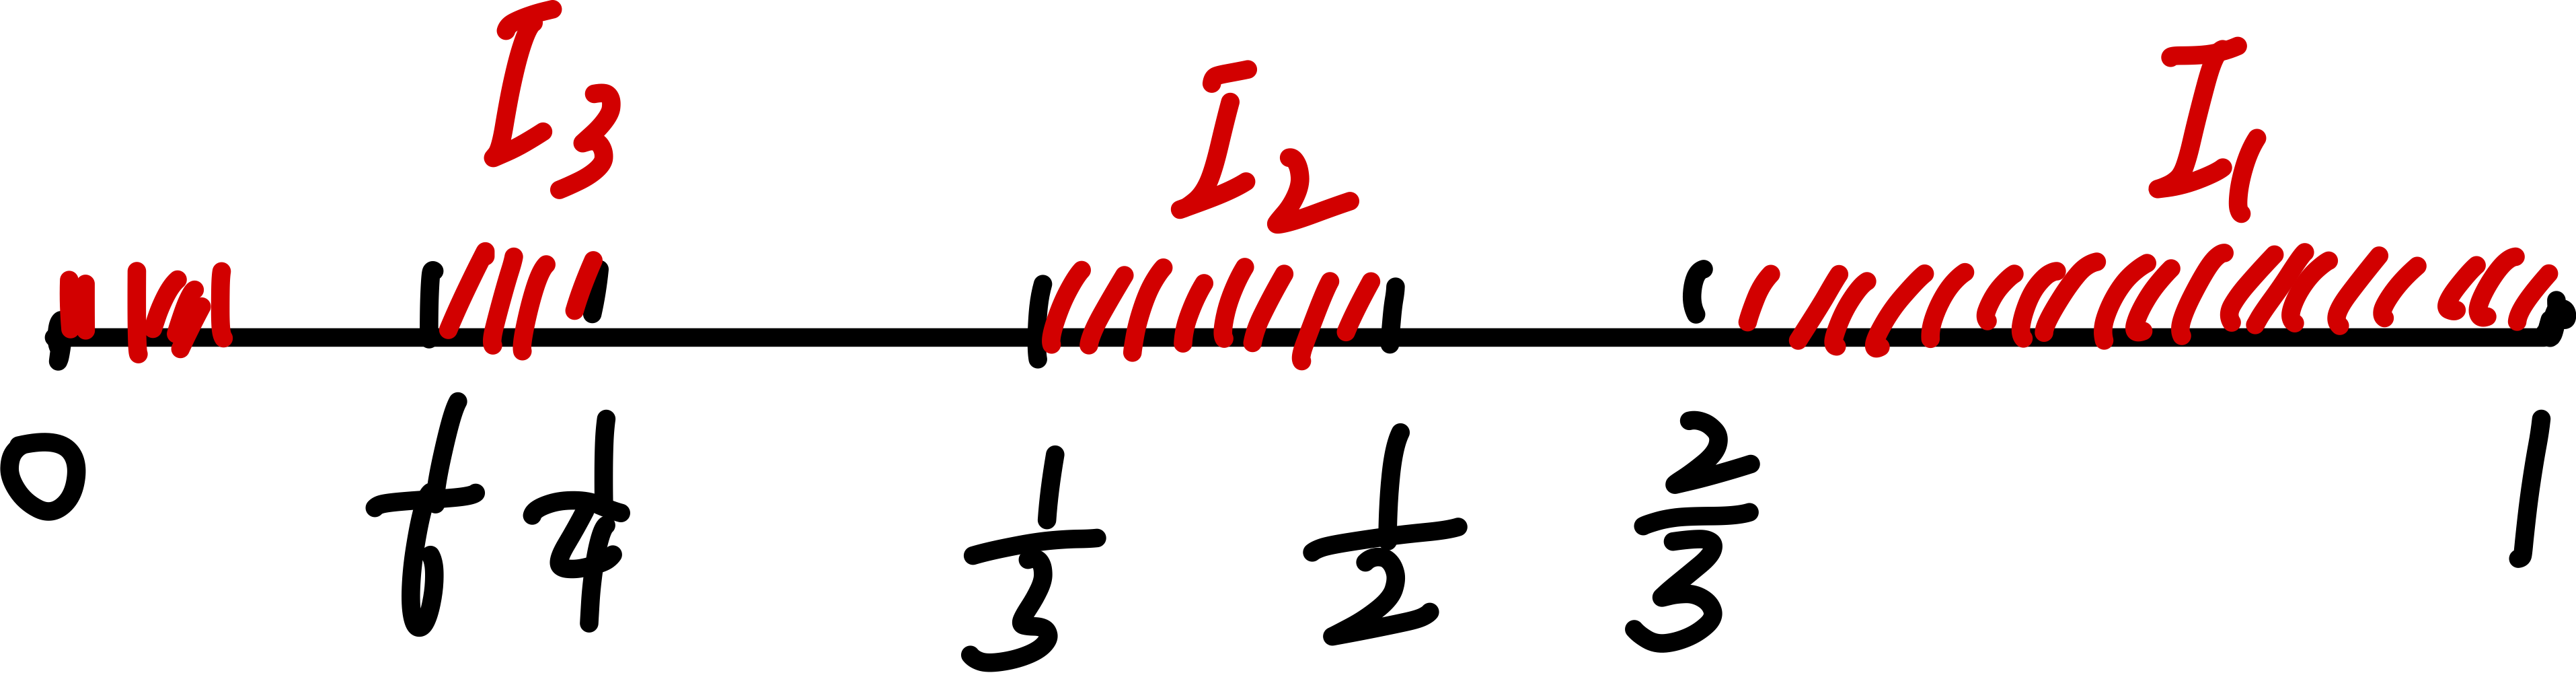
\includegraphics[width=0.4\linewidth,height=\textheight,keepaspectratio]{assets/main--figure-raster-024.png}

\end{center}

If we take \(r_{k} = \frac{1}{2^{k}}\) for \(k \in {\mathbb{N}}\), we have:

\[B\left( {0,r_{k}} \right) = \left( {- r_{k},r_{k}} \right) = \left( {- \frac{1}{2^{k}},\frac{1}{2^{k}}} \right)\]

Then for each \(k\),

\[m(I \cap B(0,r_{k}) = \sum\limits_{j = k}^{\infty}\frac{1}{3} \cdot \frac{1}{2^{j}} = \frac{1}{3} \cdot \sum\limits_{j = k}^{\infty}\frac{1}{2^{j}} = \frac{1}{3} \cdot \frac{1}{2^{k - 1}},\quad m(B\left( {0,r_{k}} \right)) = 2r_{k} = \frac{2}{2^{k}}\]

So for each \(k\),

\[\frac{\mu(B(0,r_{k}))}{m(B(0,r_{k}))} = \frac{1}{3}\]

so we have:

\[\bar{f}(0) \geq \frac{1}{3}\]

But if we take \(r_{k} = \frac{2}{3} \cdot \frac{1}{2^{k}}\), then for each \(k\),

\[m(I \cap B(0,r_{k})) = \sum\limits_{j = k + 1}^{\infty}\frac{1}{3} \cdot \frac{1}{2^{j}} = \frac{1}{3} \cdot \sum\limits_{j = k + 1}^{\infty}\frac{1}{2^{j}} = \frac{1}{3} \cdot \frac{1}{2^{k}},\quad m(B\left( {0,r_{k}} \right)) = 2r_{k} = \frac{2}{2^{k}}\]

So for each \(k\),

\[\frac{\mu(B(0,r_{k}))}{m(B(0,r_{k}))} = \frac{1}{6}\]

so we have:

\[\underset{¯}{f}(0) \leq \frac{1}{6}\]

Proving that

\[\bar{f}(0) \neq \underset{¯}{f}(0)\]

This serves as an counterexample of \(A \neq {\mathbb{R}}^{n}\) (\(n = 1\) here)

\end{example}

\section{\texorpdfstring{Lebesgue decomposition \(\left. \nu = \lambda + \rho\Longrightarrow \middle| \nu \middle| = \middle| \lambda \middle| + \middle| \rho| \right.\)}{Lebesgue decomposition \textbackslash left. \textbackslash nu = \textbackslash lambda + \textbackslash rho\textbackslash Longrightarrow \textbackslash middle\textbar{} \textbackslash nu \textbackslash middle\textbar{} = \textbackslash middle\textbar{} \textbackslash lambda \textbackslash middle\textbar{} + \textbackslash middle\textbar{} \textbackslash rho\textbar{} \textbackslash right.}}\label{lebesgue-decomposition-nulambdarhoimplies-nulambdarho}

\begin{itemize}
\item
  Let \(\nu\) be a regular complex or finite signed Borel measure on \({\mathbb{R}}^{n}\), and let \(\nu = \lambda + \rho\) be its Lebesgue decomposition with respect to Lebesgue measure \(m\), so that \(\lambda \perp m\) and \(\rho \ll m\). Prove that the Lebesgue decomposition of the total variation measure \(|\nu|\) with respect to \(m\) is given by \(\left. |\nu \middle| = \middle| \lambda \middle| + \middle| \rho| \right.\). In other words, prove that \(\left. |\nu \middle| = \middle| \lambda \middle| + \middle| \rho| \right.\), \(\left. |\lambda \middle| \perp m \right.\), and \(\left. |\rho \middle| \ll m \right.\).
\item
  Let \(\mu_{1}\) and \(\mu_{2}\) be positive, mutually singular Borel measures on \({\mathbb{R}}^{n}\). Prove that \(\mu_{1} + \mu_{2}\) is regular iff \(\mu_{1}\) and \(\mu_{2}\) are both regular.
\end{itemize}

\emph{Remark}: these results were used the the proof of Theorem 3.22 in Folland. Please don't use any results from~§7.

\begin{proof}

\textbf{of (a):} Recall that for two complex measures \(\lambda,\rho\), we define they are mutually singular if:

\[\lambda \perp \rho\quad\Leftrightarrow\quad\lambda_{r} \perp \rho_{r},\quad\lambda_{r} \perp \rho_{i},\quad\lambda_{i} \perp \rho_{r},\quad\lambda_{i} \perp \rho_{i}\]

We first show an equivalent form of it, for further use.\\

% qlnotes: kind=lemma; id=lem-hw11-on-regular-borel-measure-bv-lemma-003; concepts=lemma-003
\begin{lemma}\label{lem-hw11-on-regular-borel-measure-bv-lemma-003}

For two complex measures \(\lambda,\rho\)

\[\left. \lambda \perp \rho\quad\Leftrightarrow\quad\exists A \in \mathcal{A}\text{s.t.} \middle| \lambda \middle| (A^{c}) = 0\ \text{and} \middle| \rho \middle| (A) = 0\quad\Leftrightarrow\quad \middle| \lambda \middle| \perp \middle| \rho| \right.\]

\end{lemma}

\textbf{Proof of the lemma:} The second equivalence follows from definition (since total variation measure is positive), and the backward direction of the first equivalence follows from that the null set of the total variation measure is also the null set for original complex measure (thus null set for the positive and imaginary part).\\
For the forward direction of the first equivalence,

\[\begin{matrix}
{\lambda_{a} \perp \rho_{b}} & {\Longrightarrow\exists A_{ab} \in \mathcal{A}:A_{ab}\ \text{is null set for}\ \rho_{b}\ \text{and}\ A_{ab}^{c}\ \text{is null set for}\ \lambda_{a}} \\
 & \left. \Longrightarrow\exists A_{ab} \in \mathcal{A}: \middle| \lambda_{a} \middle| \left( A_{ab}^{c} \right) = 0, \middle| \rho_{b} \middle| \left( A_{ab} \right) = 0 \right.
\end{matrix}\]

Define:

\[A := (A_{rr} \cap A_{ri})\bigcup(A_{ir} \cap A_{ii}) \in \mathcal{A}\]

Since \(A_{rr} \cap A_{ri}\) is a null set for \(\rho_{r},\rho_{i}\), thus a null set for \(|\rho|\). And \((A_{rr} \cap A_{ri})^{c} = A_{rr}^{c} \cup A_{ri}^{c}\). Since these two are both null set for \(\lambda_{r}\) and union of null sets is null set, \((A_{rr} \cap A_{ri})^{c}\) is also a null set for \(\lambda_{r}\).\\
Similarly, \(A_{ir} \cap A_{ii}\) is a null set for \(|\rho|\) and \((A_{ir} \cap A_{ii})^{c}\) is a null set for \(\lambda_{i}\).\\
Thus, \(A\) is a null set for \(|\rho|\), and \(A^{c} = (A_{rr} \cap A_{ri})^{c}\bigcap(A_{ir} \cap A_{ii})^{c}\) is a null set for both \(\lambda_{r}\) and \(\lambda_{i}\), thus a null set for \(\lambda\).\\
This finishes the construction of \(A\), proving our lemma. Now we can apply the equivalent conditions of \(\lambda \perp \rho\) for positive, signed and complex measures.\\
Now we prove this statement which immediately implies what we want:

% qlnotes: kind=proposition; id=prop-hw11-on-regular-borel-measure-bv-proposition-001; concepts=proposition-001
\begin{proposition}\label{prop-hw11-on-regular-borel-measure-bv-proposition-001}

If complex measure \(\lambda\) and \(\rho\) on the same measurable space are mutually singular, then

\[\left. |\lambda + \rho \middle| = \middle| \lambda \middle| + \middle| \rho| \right.\]

\end{proposition}

\textbf{Proof of Proposition:} Since \(\lambda \perp \rho\), there exists a measurable set \(A \subseteq X\) such that:

\[\left. |\lambda \middle| \left( A^{c} \right) = 0\quad\text{and}\quad \middle| \rho \middle| (A) = 0 \right.\]

Let \(\nu := \lambda + \rho\). Let \(E \in \mathcal{A}\).

Then

\[\begin{matrix}
\left. |\nu \middle| (E) = \middle| \nu \middle| ((E \cap A) \sqcup (E \cap A^{c})) \right. & \left. = \middle| \nu \middle| (E \cap A) + \middle| \nu \middle| (E \cap A^{c}) \right. & \\
 & \left. = \middle| \lambda + \rho \middle| (E \cap A) + \middle| \lambda + \rho \middle| (E \cap A^{c}) \right. & \\
 & \left. = \middle| \lambda \middle| (E \cap A) + \middle| \rho \middle| (E \cap A^{c})\quad \right. & {\text{since}\ \lambda = 0\ \text{on}\ A^{c}\ \text{and}\ \rho = 0\ \text{on}\ A} \\
 & \left. = \middle| \lambda \middle| (E) + \middle| \rho \middle| (E)\quad \right. & {\text{since}\left| \lambda \middle| \text{is}\ 0\ \text{on}\ E \cap A^{c}\ \text{,} \middle| \rho \middle| \text{is}\ 0\ \text{on}\ E \cap A \right.}
\end{matrix}\]

finishing the proof the the proposition.\\
Now we look back at the original statement: For Lebesgue decomposition \(\nu = \lambda + \rho\), we have \(\lambda \perp m\) and \(\rho \ll m\). \(\lambda \perp m\) implies that there exists a measurable set \(A \subseteq X\) such that:

\[\left. |\lambda \middle| (A^{c}) = 0\quad\text{and}\quad m(A) = 0 \right.\]

Since \(\rho \ll m\), null sets of \(m\) are also null sets of \(\rho\), thus \(\left. |\rho \middle| (A) = 0 \right.\). Thus we have

\[\lambda \perp \rho\]

By our just proved proposition we have:

\[\left. |\nu \middle| = \middle| \lambda + \rho \middle| = \middle| \lambda \middle| + \middle| \rho| \right.\]

And it also follows from our lemma that

\[\left. \lambda \perp m\Longrightarrow \middle| \lambda \middle| \perp m \right.\]

and \(\left. |\rho \middle| \ll m \right.\) is trivial, since \(|\rho|\) and \(\rho\) have the same null sets.\\
This finishes the proof that: \textbf{if Lebesgue decomposition of \(\nu\) is \(\nu = \lambda + \rho\), then Lebesgue decomposition of the total variation measure \(|\nu|\) with respect to \(m\) is given by \(\left. |\nu \middle| = \middle| \lambda \middle| + \middle| \rho| \right.\).}

\end{proof}

\begin{proof}

\textbf{of (b):} \textbf{First we show (\(\Longrightarrow\):) if \(\mu_{1}\) and \(\mu_{2}\) are both regular then \(\mu_{1} + \mu_{2}\) is regular.}\\
Let \(A\) be a Borel set. Since \(\mu_{1}\) and \(\mu_{2}\) are regular, we have:

\[\mu_{1}(A) = \inf\limits_{A \subset U}\mu_{1}(U) = \sup\limits_{K \subset A}\mu_{1}(K),\quad\mu_{2}(A) = \inf\limits_{A \subset U}\mu_{2}(U) = \sup\limits_{K \subset A}\mu_{2}(K)\]

Set \(\mu = \mu_{1} + \mu_{2}\), then

\[\mu(A) = \inf\limits_{A \subset U}(\mu(U)) = \inf\limits_{A \subset U}(\mu_{1}(U) + \mu_{2}(U)) \geq \inf\limits_{A \subset U}\mu_{1}(U) + \inf\limits_{A \subset U}\mu_{2}(U) = \mu_{1}(A) + \mu_{2}(A)\]

Also on the other direction,

\[\mu(A) = \sup\limits_{K \subset A}(\mu(K)) = \sup\limits_{K \subset A}\mu_{1}(K) + \mu_{2}(K)) \leq \sup\limits_{K \subset A}\mu_{1}(K) + \sup\limits_{K \subset A}\mu_{2}(K) = \mu_{1}(A) + \mu_{2}(A)\]

Combining these two ineq chains, all inequalities is indeed equality. Thus we have

\[\mu(A) = \inf\limits_{A \subset U}(\mu(U)) = \sup\limits_{K \subset A}(\mu(K)) = \mu_{1}(A) + \mu_{2}(A)\]

The first two equalities shows regularities, and the last equality shows finiteness. This finishes the proof of forward direction.\\
\textbf{Next we show: (\(\Longleftarrow\):) if \(\mu_{1} + \mu_{2}\) is regular then \(\mu_{1}\) and \(\mu_{2}\) are both regular.}\\
Let \(A\) be a Borel set.\\
First, suppose \(A\) is compact. Then \((\mu_{1} + \mu_{2})(K) < \infty\). Notice, since \(\mu_{1},\mu_{2}\) are positive measures, \(\mu_{1} + \mu_{2} \geq \mu_{1},\mu_{2}\), thus we sure have

\[\mu_{1}(A),\mu_{2}(A) < \infty\]

This shows the \textbf{local finiteness} of \(\mu_{1},\mu_{2}\). It \textbf{remains to show the outer regularity} of \(\mu_{1},\mu_{2}\). (Note: local finiteness \(\Longrightarrow\) outer regularity is reached using tools in Ch7, so we still need to show outer regularity here; for local finiteness + outer regularity \(\Longrightarrow\) inner regularity, it have similar steps as Thm 1.18, so it is done.)\\
Since \(\mu_{1} \perp \mu_{2}\), there exists measurable \(E \subset {\mathbb{R}}^{n}\) s.t.

\[E\ \text{null for}\ \mu_{1},\quad E^{c}\ \text{null for}\ \mu_{2}\]

By outer regularity of \(\mu_{1} + \mu_{2}\), we can construct a seq of open sets \(U_{k} \supset A\) s.t.

\[(\mu_{1} + \mu_{2})(U_{k}) < (\mu_{1} + \mu_{2})(A) + \frac{1}{2^{k}}\]

Thus we have

\[\lim\limits_{k\rightarrow\infty}(\mu_{1} + \mu_{2})(U_{k}) = (\mu_{1} + \mu_{2})(A)\]

And notice that, for each \(k\),

\[\begin{matrix}
{(\mu_{1} + \mu_{2})(U_{k})} & {= (\mu_{1} + \mu_{2})(U_{k} \cap E) + (\mu_{1} + \mu_{2})(U_{k} \cap E^{c})} & \\
 & {= \mu_{1}(U_{k} \cap E^{c}) + \mu_{2}(U_{k} \cap E)\ } & {\text{since}\ E\ \text{null for}\ \mu_{1}, E^{c}\ \text{null for}\ \mu_{2}}
\end{matrix}\]

And for \(A\), similarly we have:

\[(\mu_{1} + \mu_{2})(A) = \mu_{1}(A \cap E^{c}) + \mu_{2}(A \cap E)\]

Since \(U_{k} \supset A\), we have \(U_{k} \cap E \supset A \cap E\), thus \(\mu_{1}(U_{k} \cap E^{c}) \geq \mu_{1}(A \cap E^{c})\), and similarly \(\mu_{2}(U_{k} \cap E) \geq \mu_{2}(A \cap E)\).\\
Thus

\[\begin{matrix}
 & {\quad(\mu_{2} + \mu_{2})(U_{k}) - (\mu_{2} + \mu_{2})(A)} & \\
 & {= \mu_{1}(U_{k} \cap E^{c}) + \mu_{2}(U_{k} \cap E) - (\mu_{1}(A \cap E^{c}) + \mu_{2}(A \cap E))} & \\
 & {= \mu_{1}(U_{k} \cap E^{c}) - \mu_{1}(A \cap E^{c}) + (\mu_{2}(U_{k} \cap E) - \mu_{2}(A \cap E))} & \\
 & {\geq \mu_{1}(U_{k} \cap E^{c}) - \mu_{1}(A \cap E^{c})\ } & {\text{(since}\ \mu_{2}(U_{k} \cap E) - \mu_{2}(A \cap E) \geq 0\ \text{)}} \\
 & {= \mu_{1}(U_{k} \cap E^{c}) + \mu_{1}(U_{k} \cap E) - \mu_{1}(A \cap E^{c}) - \mu_{1}(A \cap E)\ } & {\text{(since}\ \mu_{1}(U_{k} \cap E),\mu_{2}(A \cap E) = 0\ \text{)}} \\
 & {= \mu_{1}(U_{k}) - \mu_{1}(A) \geq 0} &
\end{matrix}\]

Therefore

\[(\mu_{1} + \mu_{2})(U_{k})\operatorname{\searrow ︎}\limits^{k\rightarrow\infty}(\mu_{1} + \mu_{2})(A)\Longrightarrow\mu_{1}(U_{k})\operatorname{\searrow ︎}\limits^{k\rightarrow\infty}\mu_{1}(A)\]

Since \(U_{k} \supset A\) for each \(k\), this shows the outer regularity:

\[\mu_{1}(A) = \inf\limits_{U\ \text{open}\  \supset A}\mu_{1}(U)\]

And dually, through exact same steps we can get:

\[\mu_{2}(U_{k})\operatorname{\searrow ︎}\limits^{k\rightarrow\infty}\mu_{2}(A),\quad\mu_{2}(A) = \inf\limits_{U\ \text{open}\  \supset A}\mu_{2}(U)\]

finishing the proof.

\end{proof}

\section{A convergence problem}\label{a-convergence-problem}

Let \(f \in L^{1}({\mathbb{R}})\). For \(n \in {\mathbb{N}}\), define \(f_{n}:{\mathbb{R}}\rightarrow{\mathbb{R}}\) as follows. For \(k \in {\mathbb{Z}}\) and \(x \in \lbrack\frac{k}{n},\frac{k + 1}{n})\), set

\[f_{n}(x) := n\int_{\frac{k}{n}}^{\frac{k + 1}{n}}f(t)\, dt\]

\begin{itemize}
\item
  Prove that \(f_{n}\rightarrow f\) a.e.
\item
  Prove that \(f_{n}\rightarrow f\) in \(L^{1}\).
\end{itemize}

\emph{Hint}: for (a), use the Lebesgue differentiability theorem; for (b) you may want to approximate \(f\) by a nice function.

\begin{proof}

\textbf{of (a):}

\begin{center}

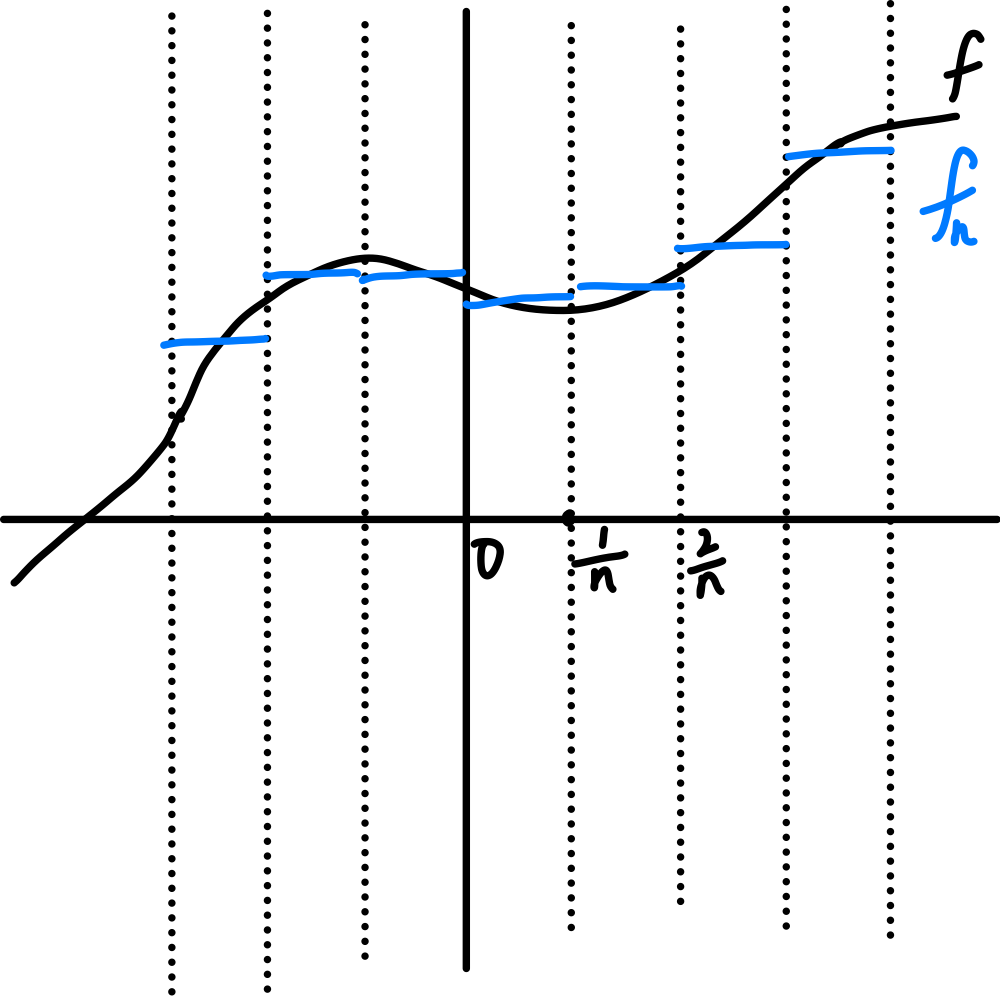
\includegraphics[width=0.3\linewidth,height=\textheight,keepaspectratio]{assets/main--figure-raster-037.png}

\end{center}

\[f_{n}(x) = n\int_{\frac{k}{n}}^{\frac{k + 1}{n}}f(t)\, dt = \frac{1}{1/n}\int_{I_{n,k}}f(t)\, dt = \frac{1}{m(I_{n,k})}\int_{I_{n,k}}f(t)\, dt\]

Thus \(f_{n}(x)\) is the average of \(f\) over the interval \(I_{n,k} := \left\lbrack {\frac{k}{n},\frac{k + 1}{n}} \right)\), where \(x \in I_{n,k}\).\\
Fixing \(x \in {\mathbb{R}}\), for each \(n\) we set \(E_{n}(x) := I_{n,k}\) for \(I_{n,k}\) s.t. \(x \in I_{n,k}\). Notice that for each \(n\),

\[\bigsqcup\limits_{k}I_{n,k} = {\mathbb{R}}\]

so this \(E_{n}\) is well-defined.\\
And for each \(E_{n}\), we have

\[E_{n}(x) = \left\lbrack {\frac{k}{n},\frac{k + 1}{n}} \right) \subset \left( {x - \frac{2}{n},x + \frac{2}{n}} \right) = B(x,\frac{2}{n})\]

And

\[m(E_{n}(x)) = \frac{1}{n} = \frac{1}{4}m(B(x,\frac{2}{n}))\]

This shows that \textbf{\(E_{n}(x)\) nicely shrinks to \(x\) as \(n\rightarrow\infty\).} Then by LDT, we have

\[\lim\limits_{n\rightarrow\infty}f_{n}(x) = \lim\limits_{n\rightarrow\infty}\frac{1}{m(E_{n}(x))}\int_{E_{n}(x)}f(t)\, dt = f(x)\]

for \(m\)-a.e. \(x\).\\
This finishes the proof.

\end{proof}

\begin{proof}

\textbf{of (b):} WTS:

\[\left. \lim\limits_{n\rightarrow\infty} \parallel f_{n} - f\underset{1}{\parallel} = \int \middle| f_{n}(x) - f(x) \middle| \, dx = 0 \right.\]

Since \(f \in L^{1}({\mathbb{R}})\), we can select \(\phi \in C_{c}^{0}({\mathbb{R}})\) a ctn compactly supported function (e.g., can take bump function) such that

\[\parallel f - \phi\underset{1}{\parallel} < \varepsilon/3\]

Now define \(\phi_{n}\) by averaging \(\phi\) over the same intervals:

\[\phi_{n}(x) := n\int_{k/n}^{(k + 1)/n}\phi(t)\, dt = \frac{1}{m(I_{n,k})}\int_{I_{n,k}}\phi(t)\, dt\quad\text{, for}\ x \in \left\lbrack {\frac{k}{n},\frac{k + 1}{n}} \right)\]

Then by tri eq on \(L^{1}(m)\),

\[\parallel f_{n} - f\underset{1}{\parallel} \leq \parallel f_{n} - \phi_{n}\underset{1}{\parallel} + \parallel \phi_{n} - \phi\underset{1}{\parallel} + \parallel \phi - f\underset{1}{\parallel}\]

First, \(\parallel \phi - f\underset{1}{\parallel} < \varepsilon/3\) by construction. Next, fixing \(n,k\), we write the value of \(f_{n}(x)\) over the interval \(I_{n,k} := \left\lbrack {\frac{k}{n},\frac{k + 1}{n}} \right)\) as \(f_{n,k}\), and value of \(\phi_{n}(x)\) over the interval \(I_{n,k} := \left\lbrack {\frac{k}{n},\frac{k + 1}{n}} \right)\) as \(\phi_{n,k}\). Then for each \(n,k\)

\[\begin{matrix}
\left. \parallel f_{n} \middle| {}_{I_{n,k}} - \phi_{n} \middle| {}_{I_{n,k}}\underset{1}{\parallel} \right. & \left. = \int_{I_{n,k}} \middle| f_{n,k} - \phi_{n,k} \middle| \, dx \right. \\
 & \left. = \frac{1}{n} \middle| f_{n,k} - \phi_{n,k}| \right. \\
 & \left. = \frac{1}{n} \cdot n\  \middle| \int_{I_{n,k}}(f(t) - \phi(t))\, dt\ | \right. \\
 & \left. = \middle| \int_{I_{n,k}}(f(t) - \phi(t))\, dt\ | \right.
\end{matrix}\]

Since \(\left. f_{n} - \phi_{n} = \sum_{k \in {\mathbb{Z}}}f_{n} \middle| {}_{I_{n,k}} - \phi_{n}|_{I_{n,k}} \right.\), by Minkowski's ineq we then have:

\[\begin{matrix}
{\parallel f_{n} - \phi_{n} \parallel} & \left. \leq \sum\limits_{k \in {\mathbb{Z}}} \parallel f_{n} \middle| {}_{I_{n,k}} - \phi_{n} \middle| {}_{I_{n,k}}\underset{1}{\parallel} \right. \\
 & \left. = \sum\limits_{k \in {\mathbb{Z}}} \middle| \int_{I_{n,k}}(f(t) - \phi(t))\, dt\ | \right. \\
 & \left. \leq \sum\limits_{k \in {\mathbb{Z}}}\int_{I_{n,k}} \middle| f(t) - \phi(t) \middle| \, dt \right. \\
 & \left. = \int \middle| f(t) - \phi(t) \middle| \, dt = \parallel f - \phi\underset{1}{\parallel} < \frac{\epsilon}{3} \right.
\end{matrix}\]

This shows that, for every \(n \in {\mathbb{N}}\), we all have \(\parallel f_{n} - \phi_{n} \parallel < \frac{\epsilon}{3}\).\\
And finally for \(\phi_{n} - \phi\), since \(\phi \in C_{c}^{0}({\mathbb{R}}) \subset L^{1}({\mathbb{R}})\), by (a) we already have \(\phi_{n}\rightarrow\phi\) a.e.; and, since \(\phi\) have compact support, say \(K\) with \(m(K) < \infty\) and it is continuous on the compact support, it is uniformly continuous and bounded. Say \(\left. |\phi \middle| < M \right.\) for some \(M > 0\).\\
Then the function \(g = M\) on \(K\) and \(g = 0\) on \(K^{c}\) can serve as a dominating function for \(\phi_{n}\), with \(\int g = M \cdot m(K) < \infty\). Then by DCT, we have: \(\varphi_{n}\rightarrow\varphi\) in \(L^{1}\).\\
So for some \(N \in {\mathbb{N}}\), \(\parallel \phi_{n} - \phi\underset{1}{\parallel} < \epsilon/3\) for all \(n \geq N\).\\
Therefore for all \(n \geq N\), we have:

\[\parallel f_{n} - f\underset{1}{\parallel} \leq \parallel f_{n} - \phi_{n}\underset{1}{\parallel} + \parallel \phi_{n} - \phi\underset{1}{\parallel} + \parallel \phi - f\underset{1}{\parallel} < \epsilon\]

This finishes the proof that

\[\lim\limits_{n\rightarrow\infty} \parallel f_{n} - f\underset{1}{\parallel} = 0\]

\end{proof}

\section{\texorpdfstring{Oscillations: \(F(x) = x\sin\frac{1}{x},x^{2}\sin\frac{1}{x^{2}} \in BV(I)\Leftrightarrow 0 \notin I\)}{Oscillations: F(x) = x\textbackslash sin\textbackslash frac\{1\}\{x\},x\^{}\{2\}\textbackslash sin\textbackslash frac\{1\}\{x\^{}\{2\}\} \textbackslash in BV(I)\textbackslash Leftrightarrow 0 \textbackslash notin I}}\label{oscillations-fxxsinfrac1xx2sinfrac1x2in-bvi-iff-0not-in-i}

\begin{itemize}
\item
  Define \(F:{\mathbb{R}}\rightarrow{\mathbb{R}}\) by \(F(x) = x\sin\frac{1}{x}\) for \(x \neq 0\) and \(F(0) = 1\). Prove that if \(I = \lbrack a,b\rbrack \subset {\mathbb{R}}\) is a compact interval, so that \(- \infty < a < b < \infty\), then \(F \in BV(I)\) iff \(0 \notin I\).
\item
  Define \(F:{\mathbb{R}}\rightarrow{\mathbb{R}}\) by \(F(x) = x^{2}\sin\frac{1}{x^{2}}\) for \(x \neq 0\) and \(F(0) = 0\). Prove that \(F\) is differentiable everywhere (including at \(x = 0\)) but that \(F \notin BV(\lbrack - 1,1\rbrack)\).
\end{itemize}

\begin{proof}

\textbf{of (a):}\\
\textbf{We first verify (\(\Longrightarrow\)): if \(0 \notin I\) then \(F \in BV(I)\).}\\
We differentiate \(F(x) = x\sin(1/x)\) for \(x \neq 0\):

\[F'(x) = \frac{d}{dx}\left( {x \cdot \sin\left( \frac{1}{x} \right)} \right) = \sin\left( \frac{1}{x} \right) + x \cdot \cos\left( \frac{1}{x} \right) \cdot \left( {- \frac{1}{x^{2}}} \right) = \sin\left( \frac{1}{x} \right) - \frac{1}{x}\cos\left( \frac{1}{x} \right)\]

WLOG suppose \(a > 0\), then on \(\lbrack a,b\rbrack\) we have:

\[\left. 0 \leq \middle| F' \middle| \leq 1 + \frac{1}{a} \right.\]

Then for arbitrary division of \(\lbrack a,b\rbrack\), say \(a = x_{0} \leq \cdots \leq x_{n} = b\), for all \(j\) we have:

\[\left. |F(x_{j}) - F(x_{j - 1}) \middle| \leq (1 + \frac{1}{a})(x_{j} - x_{j - 1}) \right.\]

Thus

\[\left. \sum\limits_{j = 1}^{n} \middle| F(x_{j}) - F(x_{j - 1}) \middle| \leq (1 + \frac{1}{a})(b - a) = b - a + \frac{b}{a} - 1 \right.\]

Taking sup over all partition of \(\lbrack a,b\rbrack\), proving that \(T_{F}(a;b) \leq b - a + \frac{b}{a} - 1\), proving that \(F \in BV(\lbrack a,b\rbrack)\); If \(a < 0\) then \(b < 0\) also, then \(\left. 0 \leq \middle| F' \middle| \leq 1 - \frac{1}{b} \right.\), by same reasoning showing that \(F \in BV(\lbrack a,b\rbrack)\).\\
\textbf{Then we verify: (\(\Longleftarrow\)): if \(F \in BV(I)\) then \(0 \notin I\). This is equiv to: if \(0 \in I\) then \(F \notin BV(I)\).}\\
Suppose \(0 \in I = \lbrack a,b\rbrack\) then \(a \leq 0\) and \(b \geq 0\), one of which is strict. WLOG we suppose \(b > 0\).\\
Consider this seq:

\[y_{n} := \frac{1}{n\pi + \pi/2}\rightarrow 0^{+}\]

we have:

\[F\left( y_{n} \right) = y_{n}\sin\left( \frac{1}{y_{n}} \right) = \frac{1}{n\pi + \pi/2} \cdot \sin(n\pi + \pi/2)\]

For odd \(n\), \(F(y_{n}) = \frac{- 1}{n\pi + \pi/2}\), for even \(n\), \(F(y_{n}) = \frac{1}{n\pi + \pi/2}\).\\
Since \(b > 0\), for some \(N_{0}\) we have \(y_{N_{0}} < b\). Then we consider the partition: pick \(N \in {\mathbb{N}}\), and use \(x_{0} = 0,x_{1} = y_{N_{0} + N - 1},x_{2} = y_{N_{0} + N - 2},\cdots,x_{N} = y_{N_{0}},x_{N + 1} = b\) as the partition points of \(\lbrack 0,b\rbrack\).\\
Then we have

\[\left. \sum\limits_{n = 1}^{N + 1} \middle| F(x_{n}) - F(x_{n - 1}) \middle| \geq \sum\limits_{n = N_{0}}^{N_{0} - 2 + N}\frac{1}{\pi n + \pi/2} + \frac{1}{\pi(n + 1) + \pi/2} \geq 2\sum\limits_{n = N_{0}}^{N_{0} - 2 + N}\frac{1}{\pi n + \pi/2} \right.\]

As \(N\rightarrow\infty\), this sum \(\left. \sum_{n = 1}^{N + 2} \middle| F(x_{j}) - F(x_{j - 1}) \middle| \rightarrow\infty \right.\), by the harmonic series. Then taking sup over all partitions, the sup is unbounded, showing that \(F \notin BV(\lbrack 0,b\rbrack)\), thus \(F \notin BV(I)\). Same reasoning when we suppose \(a < 0\) is strict.

\end{proof}

\begin{proof}

\textbf{of (b):} \textbf{For \(x \neq 0\):} \(\sin(1/x^{2})\) is differentiable as the composition of two differentiable functions, thus differentiable; and \(F(x) = x^{2}\sin\left( {1/x^{2}} \right)\) is the product of differentiable functions, so \(F\) is differentiable.\\
\textbf{For \(x = 0\):}

\[\lim\limits_{x\rightarrow 0}\frac{F(x) - F(0)}{x - 0} = \lim\limits_{x\rightarrow 0}\frac{x^{2}\sin\left( \frac{1}{x^{2}} \right)}{x} = \lim\limits_{x\rightarrow 0}x\sin\left( \frac{1}{x^{2}} \right)\]

Since \(\left| {\sin\left( {1/x^{2}} \right)} \right| \leq 1\), we get \(\left. \left| {x\sin\left( {1/x^{2}} \right)} \right| \leq \middle| x \middle| \rightarrow 0 \right.\) as \(x\rightarrow 0\), thus \(F\) is differentiable at \(x = 0\), and \(F'(0) = 0\).\\
This proves that, \(F\) is differentiable everywhere on \(\mathbb{R}\).\\
Now we show that \(F \notin BV(\lbrack - 1,1\rbrack)\):\\
Consider this seq:

\[y_{n} := \sqrt{\frac{1}{n\pi + \pi/2}}\rightarrow 0^{+}\]

we have:

\[F\left( y_{n} \right) = y_{n}^{2}\sin\left( \frac{1}{y_{n}^{2}} \right) = \frac{1}{n\pi + \pi/2} \cdot \sin(n\pi + \pi/2)\]

For odd \(n\), \(F(y_{n}) = \frac{- 1}{n\pi + \pi/2}\), for even \(n\), \(F(y_{n}) = \frac{1}{n\pi + \pi/2}\).\\
Notice that \(y_{1} < 1\), so we then consider the partition: pick \(N \in {\mathbb{N}}\), and use \(x_{0} = 0,x_{1} = y_{N},x_{2} = y_{N - 1},\cdots,x_{N} = y_{1},x_{N + 1} = 1\) as the partition points of \(\lbrack 0,1\rbrack\).\\
Then we have

\[\begin{matrix}
{T_{F}(1) - T_{F}( - 1)} & \left. \geq \sum\limits_{n = 1}^{N + 1} \middle| F(x_{n}) - F(x_{n - 1})| \right. \\
 & \left. \geq \sum\limits_{n = 2}^{N} \middle| F(y_{n}) - F(y_{n - 1})| \right. \\
 & {\geq \sum\limits_{n = 2}^{N}\frac{1}{\pi n + \pi/2} + \frac{1}{\pi(n - 1) + \pi/2}} \\
 & {\geq 2\sum\limits_{n = 2}^{N}\frac{1}{\pi n + \pi/2}}
\end{matrix}\]

This sum is unbounded as \(N\rightarrow\infty\) by the harmonic series. Then taking sup over all partitions, the sup is unbounded, showing that \(F \notin BV(\lbrack - 1,1\rbrack)\).

\end{proof}

\section{Everywhere unbounded variation}\label{everywhere-unbounded-variation}

Construct a function \(F \in C_{0}^{0}({\mathbb{R}})\) (see HW9) such that \(F\) does not have bounded variation on any interval \(\lbrack a,b\rbrack\) with \(a < b\). \emph{Hint}: construct \(F\) based on functions like the ones in the previous problem.

\begin{qlsolution}{Solution}

We consider this function as the building block:

\[\begin{matrix}
{G(x) = \{ x\sin\frac{1}{x},\quad x \in ( - \frac{1}{\pi},0) \cup (0,\frac{1}{\pi})} \\
{0,\quad\text{elsewhere}}
\end{matrix}\]

We know that, this function is \textbf{continuous} (we know in elementary real analysis course that it is true for \(x \in ( - \frac{1}{\pi},\frac{1}{\pi})\), and \(G\rightarrow 0\) as \(x\rightarrow \pm - \frac{1}{\pi}\), so it is true all over the domain.) and similar reasoning as question 4(a), we can verift that, \textbf{\(G \notin BV(I)\) for any \(I \ni 0\).}\\
Also, it is clear that

\[\lim\limits_{x\rightarrow \pm \infty}G(x) = G(1) = 0\]

Thus we have:

\[G \in C_{0}^{0}({\mathbb{R}})\]

And notice this function has \textbf{uniform bound \(1\)}: setting \(t = \frac{1}{x}\), so \(x = \frac{1}{t}\), and

\[\left. |G(x) \middle| = \left| {\frac{1}{t}\sin(t)} \right| = \left| \frac{\sin(t)}{t} \right| \leq 1\quad\forall t \neq 0 \right.\]

So by translating, stretching and scaling it, we can define for each \(n\):

\[G_{n}(x) = \frac{1}{2^{n}}G(\frac{x - x_{n}}{\sigma_{n}})\]

where \textbf{we will delicately choose \(x_{n},\sigma_{n}\).}\\
By defining the partial sum seq:

\[F_{N}(x) = \sum\limits_{n = 1}^{N}G_{n}(x)\]

Then by geometric seq, such function is also uniformly bounded by \(1\), and it is continuous since it is finite sum of continuous functions, and also have \(F_{N}(x)\rightarrow 0\) as \(x\rightarrow\infty\), so for each \(N\) we have \(F_{N} \in C_{0}^{0}({\mathbb{R}})\). And \(F_{N}\) is an increasing seq (not really), so define:

\[F := \lim\limits_{N\rightarrow\infty}F_{N} = \sum\limits_{n = 1}^{\infty}G_{n}\]

Then \(F_{N}\rightarrow F\) uniformly as \(N\rightarrow\infty\). This is since \(G_{n}\) is uniformly bounded by \(\frac{1}{2^{n}}\): For \(\epsilon > 0\), there exists \(N_{0}\) s.t. \(\frac{1}{2^{N - 1}} < \epsilon\), and then for all \(M \geq N_{0}\), we have

\[\left. |F_{M}(x) - F(x) \middle| \leq \sum\limits_{N = N_{0}}^{\infty}\frac{1}{2^{N}} = \frac{1}{2^{N - 1}} < \epsilon \right.\]

Thus, we also have

\[F \in C_{0}^{0}({\mathbb{R}})\]

since it is \textbf{uniform limit of continuous functions,} and the limit to \(\pm \infty\) remains \(0\). This is regardless of the choice of \(x_{n},\sigma_{n}\) for each \(n\).\\
Then, to finish the construction, it remains for us to choose \(x_{n},\sigma_{n}\) for each \(n\), to let \(F\) have the property that \(F\) does not have bounded variation on any compact interval.\\
Let \(\left\{ x_{n} \right\}\) be the enumeration of a dense subset of \(\mathbb{R}\). e.g. Let it be the enumeration of \(\mathbb{Q}\).\\
We \textbf{inductively pick \(\sigma_{n}\)}: for each \(n\), we pick \(\sigma_{n} \in (0,1)\) s.t. for all \(1 \leq j \leq n - 1\), we have \(\left. |x_{n} - x_{j} \middle| > 2\sigma_{n} \right.\) and \(\left. |x_{n + 1} - x_{n} \middle| > 2\sigma_{n} \right.\).\\
Now let \(I = \lbrack a,b\rbrack\) be an arbitrary compact interval. WTS: \(F \notin BV(I)\).\\
By density of the seq, there exists \(x_{n}\) such that \(x_{n} \in I\).\\
We consider the subinterval:

\[I' := (x_{n} - \sigma_{n},x_{n} + \sigma_{n}) \subset I\]

This construction ensures that the \(G_{1},\cdots,G_{n - 1},G_{n + 1}\) will not have some offsetting variation such to make the variation of \(G_{n}\) interfered (suspectively finite): for each \(1 \leq j \leq n\) and \(j = n + 1\), we have:

\[G_{j} \in BV(I')\]

since \(x_{j} \notin I'\). This is by question 4(a). This means that we can ignore these terms when showing \(F \notin BV(I')\).\\
And for we know that

\[G_{n} \notin BV(I')\]

since \(x_{n} \in I\), as verified by question 4(a).\\
And for the rest \(G_{n + 2},\cdots\), \textbf{their total variation contributed to this the total variation of \(F\) on \(I\) is at most a half of \(G_{n}\) (by geometric seq).}\\
Thus the only term matters is \(G_{n}\). Since \(G_{n} \notin BV(I')\), we have \(F = \sum_{n = 1}^{\infty}G_{n} \notin BV(I')\), thus \(F \notin BV(I)\) since \(I \supset I'\).\\
This finishes the proof.\\
(Rigorous reasoning is as question 4, we construct partitions to apply harmonic seq to the variation by the partition, and \(G_{n + 2},\cdots\) can at most halve it, which does not matter.)

\end{qlsolution}
\end{document}
